\documentclass[11pt]{article}
\usepackage[margin=1in]{geometry}
\usepackage{amsmath,amssymb,amsthm}
\usepackage{graphicx}
\usepackage{microtype}
\usepackage{xcolor}
\usepackage{hyperref}
\hypersetup{colorlinks=true,linkcolor=blue!55!black,urlcolor=blue!55!black,citecolor=blue!55!black}
\newtheorem{theorem}{Theorem}
\newcommand{\R}{\mathbb{R}}
\newcommand{\D}{\mathcal{D}}
\newcommand{\Tr}{\operatorname{Tr}}
\title{A critical Besov trace obstruction\\to the endpoint extension in arXiv:1904.05420}
\author{Candidate counterexample packet}
\date{11 August 2026}

\begin{document}
\maketitle

\begin{center}
\fbox{\parbox{0.91\linewidth}{\textbf{Status:} candidate counterexample likely valid.  This is a full negative answer to the universal Besov endpoint extension in Remark~6.9, subject to human review.}}
\end{center}

\section{Source problem}

Caetano, Hewett, and Moiola prove in Proposition~6.7 of
arXiv:1904.05420v2~\cite{CHM} that, if $\Gamma$ is a $d$-set in $\R^n$,
$0<d<n$, $1<p<\infty$, $1\le q<\infty$, $m\in\mathbb N_0$, and
\[
 \frac{n-d}{p}+m<s<\frac{n-d}{p}+m+1,
\]
then
\[
 \D(\Gamma^c)\text{ is dense in }
 \ker\!\left(\Tr_{\Gamma,m}|_{B^s_{p,q}(\R^n)}\right).
\]
Here $\D(\Gamma^c)=C_c^\infty(\R^n\setminus\Gamma)$ and
$\Tr_{\Gamma,m}$ records all traces $\operatorname{tr}_\Gamma D^\beta u$
with $|\beta|\le m$.  Remark~6.9 asks whether the same conclusion holds at
the endpoint
\[
 s=\frac{n-d}{p}+m+1.
\]

\begin{center}
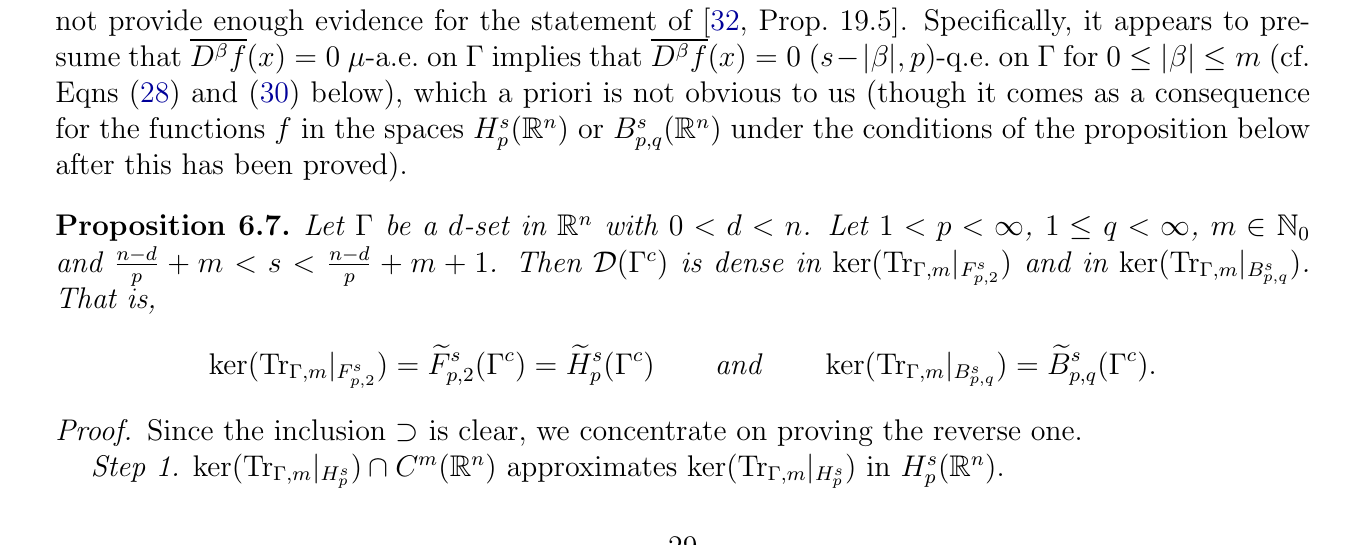
\includegraphics[width=\textwidth]{figures/proposition_context_crop.png}

\smallskip
\emph{Proposition 6.7 in the original paper, page 29.}
\end{center}

\begin{center}

\includegraphics[width=\textwidth]{figures/open_problem_crop.png}

\smallskip
\emph{The endpoint question in Remark 6.9, page 31.}
\end{center}

\section{Proof intuition}

At $q=1$, the endpoint creates one additional continuous trace.  If
$s=1/p+m+1$ for a codimension-one hyperplane, then differentiating $m+1$
times maps $B^s_{p,1}$ into the critical space $B^{1/p}_{p,1}$, whose trace
on the hyperplane is continuous.  Every function supported off the
hyperplane has this extra trace equal to zero.  But $\Tr_{\Gamma,m}$ does not
record it.  A bump times the monomial $x_n^{m+1}$ therefore lies in the
stated kernel while retaining a nonzero $(m+1)$-st normal trace.  Continuity
of that trace separates it from the claimed closure.

\section{Counterexample}

\begin{theorem}[Failure of the Besov endpoint]
Let $n\ge2$, let $\Gamma=\R^{n-1}\times\{0\}$, let $1<p<\infty$, and let
$m\in\mathbb N_0$.  Set
\[
 d=n-1,\qquad q=1,\qquad s=\frac1p+m+1
       =\frac{n-d}{p}+m+1.
\]
Then
\[
 \widetilde B^s_{p,1}(\Gamma^c)
 :=\overline{\D(\Gamma^c)}^{\,B^s_{p,1}(\R^n)}
 \subsetneq
 \ker\!\left(\Tr_{\Gamma,m}|_{B^s_{p,1}(\R^n)}\right).
\]
Consequently, the endpoint extension proposed in Remark~6.9 is false for
the class of Besov spaces stated in Proposition~6.7.
\end{theorem}

\begin{proof}
The hyperplane $\Gamma$ is an $(n-1)$-set.  Choose
$\eta\in C_c^\infty(\R^n)$ so that its restriction to $\Gamma$ is not
identically zero, write $x=(x',x_n)$, and define
\[
 u(x',x_n)=\eta(x',x_n)x_n^{m+1}.
\]
Because $u\in C_c^\infty(\R^n)$, it belongs to $B^s_{p,1}(\R^n)$.  If
$|\beta|\le m$, every term in $D^\beta u$ still contains a positive power of
$x_n$.  Hence
\[
 (D^\beta u)|_\Gamma=0\qquad (|\beta|\le m).
\]
For smooth functions the trace operator in the source is ordinary pointwise
restriction, so
\[
 u\in\ker\!\left(\Tr_{\Gamma,m}|_{B^s_{p,1}(\R^n)}\right).
\]

We show that $u$ is not in the closure of $\D(\Gamma^c)$.  Proposition~6.2
of the source gives a continuous critical trace
\[
 \operatorname{tr}_\Gamma:B^{1/p}_{p,1}(\R^n)\longrightarrow L_p(\Gamma).
\]
Since $D_n^{m+1}:B^s_{p,1}(\R^n)\to B^{1/p}_{p,1}(\R^n)$ is continuous, the
composition
\[
 \Lambda(v):=\operatorname{tr}_\Gamma(D_n^{m+1}v)
 \quad:B^s_{p,1}(\R^n)\longrightarrow L_p(\Gamma)
\]
is continuous.  Every $\varphi\in\D(\Gamma^c)$ vanishes on a neighborhood of
$\Gamma$, and therefore $\Lambda(\varphi)=0$.  It follows by continuity that
$\Lambda$ vanishes on $\widetilde B^s_{p,1}(\Gamma^c)$.

Leibniz' rule, evaluated at $x_n=0$, gives
\[
 \Lambda(u)(x')
 =\left.D_n^{m+1}\bigl(\eta(x',x_n)x_n^{m+1}\bigr)\right|_{x_n=0}
 =(m+1)!\,\eta(x',0),
\]
which is nonzero in $L_p(\Gamma)$ by the choice of $\eta$.  Thus
$u\notin\widetilde B^s_{p,1}(\Gamma^c)$, proving strict inclusion.
\end{proof}

The smallest concrete instance is $n=2$, $p=2$, $m=0$:
$\Gamma=\R\times\{0\}$, $s=3/2$, and $u(x,y)=\eta(x,y)y$.  Its value trace
is zero, while its normal trace is $\eta(x,0)\ne0$.

\section{Verification report}

The proof uses only the following checks.
\begin{enumerate}
\item The chosen hyperplane satisfies every geometric hypothesis of
Proposition~6.7 with $d=n-1$.
\item The allowed parameter $q=1$ is essential: Proposition~6.2 supplies
the continuous critical trace on $B^{1/p}_{p,1}$.
\item Leibniz' rule shows all jets through order $m$ vanish, while the pure
normal jet of order $m+1$ equals $(m+1)!\eta|_\Gamma$.
\item Continuity of $\Lambda$ makes its kernel closed and containing
$\D(\Gamma^c)$, so it contains the claimed closure but not $u$.
\end{enumerate}
There is no numerical or computational premise.  The verifier should focus on
the source's endpoint trace normalization in Proposition~6.2 and on the fact
that $q=1$ is included in Proposition~6.7.

\section{Scope and literature status}

This counterexample disproves the universal Besov endpoint extension; it does
not contradict an endpoint theorem for Bessel-potential spaces.  Hinz,
Chandler-Wilde, and Hewett later cited Remark~6.9 explicitly and gave an
affirmative answer for the fractional Sobolev spaces $H_p^s$ in their
Corollary~3.2 and Remark~3.3~\cite{HCH}.  Their paper describes the earlier
Besov result but does not claim the Besov endpoint.  Thus the two conclusions
are compatible: the Sobolev endpoint is positive, while the Besov family in
the original universal formulation already fails at $q=1$.

\section{Bounded novelty check}

The search through 11 August 2026 covered the run's registry, solution,
attempt, and proof-gap indexes; exact searches for Remark~6.9 and
Proposition~6.7; the title and arXiv identifier 1904.05420 combined with
\emph{endpoint}, \emph{trace}, \emph{Besov}, and \emph{counterexample}; and
the citing arXiv paper 2507.04536.  The last source is an explicit later
answer to the Sobolev branch, but the bounded search found no statement of
the $q=1$ Besov counterexample above.  Novelty confidence is moderate pending
a specialist search of books and non-indexed literature; mathematical
validity does not depend on novelty.

\section{Conclusion and review recommendation}

Remark~6.9 has a negative answer as a proposed extension of all conclusions
of Proposition~6.7: at the Besov endpoint with $q=1$, the next jet becomes a
continuous invariant and obstructs density.  Promotion as a likely valid
counterexample is recommended, with human verification of the critical trace
citation and a specialist novelty check.

\begin{thebibliography}{9}
\bibitem{CHM}
A. M. Caetano, D. P. Hewett, and A. Moiola,
\emph{Density results for Sobolev, Besov and Triebel--Lizorkin spaces on rough sets},
J. Funct. Anal. 281 (2021), 109019; arXiv:1904.05420v2.
\url{https://arxiv.org/abs/1904.05420}.

\bibitem{HCH}
M. Hinz, S. N. Chandler-Wilde, and D. P. Hewett,
\emph{Kernels of trace operators via fine continuity},
arXiv:2507.04536, 2025.
\url{https://arxiv.org/abs/2507.04536}.
\end{thebibliography}

\end{document}
